\documentclass[ngerman]{dtk}% load class options 07
%%
%% Packete/Style-Optionen und anderes Material in der Pr"aambel:
%%
\usepackage{showexpl}
\usepackage{ifthen}
\usepackage{xspace}
\usepackage{listings}
\usepackage{xcolor}
\usepackage{babel}
\usepackage{microtype}
\usepackage[utf8]{inputenc}
\usepackage{graphicx}
\usepackage{csquotes}
\usepackage{booktabs}
\usepackage{lmodern}

\addto\captionsngerman{\renewcommand{\refname}{Referenzen}}


\definecolor{hellgelb}{rgb}{1,1,0.8}
\definecolor{colKeys}{rgb}{0,0,1}
\definecolor{colIdentifier}{rgb}{0,0,0}
\definecolor{colComments}{rgb}{1,0,0}
\definecolor{colString}{rgb}{0,0.5,0}

\lstset{%
    float=hbp,%
    basicstyle=\ttfamily\small, %
    identifierstyle=\color{colIdentifier}, %
    keywordstyle=\color{colKeys}, %
    stringstyle=\color{colString}, %
    commentstyle=\color{colComments}, %
    columns=flexible, %
    tabsize=2, %
%    frame=single, %
    extendedchars=true, %
    showspaces=false, %
    showstringspaces=false, %
    backgroundcolor=\color{hellgelb}, %
    breakautoindent=true, %
    captionpos=b%
}

\begin{document}

\title{Spendenbescheinigungen erstellen mit \LaTeX, SQL \\ und Python}

\Author{Uwe}{Ziegenhagen}{Köln}

\maketitle

\markboth{Spendenbescheinigungen}{Spendenbescheinigungen}

%%-----------------------------------------------------------------------------
\begin{abstract}
In der Funktion als Kassenwart der Kölner Dingfabrik e.\,V. muss ich spätestens im Frühjahr eine Vielzahl von  Spendenbescheinigungen erstellen. Der bisher gelebte Prozess, die händische Aggregation der Daten in Excel und Fertigstellung von MS~Word Schreiben, war keine Option für einen überzeugten \TeX ie; eine automatisierte Lösung musste gefunden werden.

Im folgenden Artikel beschreibe ich den Workflow der Erstellung der Spendenformulare mittels \LaTeX\ sowie ihre Befüllung aus einer Datenbank über selbstgeschriebener Python-Skripte.
\end{abstract}

\section{Erstellung der Formulare}
Seit dem 01.~Januar 2013 sind vom Bundesministerium für Finanzen neue Muster für Zuwendungsbestätigungen\footnote{Beamtendeutsch für \enquote{Spendenquittungen}} vorgeschrieben.

Auf den offiziellen Webseiten\footnote{\url{http://www.finanzamt.bayern.de/Informationen/Formulare/Weitere_Themen_A_bis_Z/Spenden/default.php}}
werden leider nur Word- und PDF-Vorlagen angeboten, sodass die Vorlagen in \LaTeX\ nachgebaut werden müssen.

Als Alternative könnte man zwar die PDF Formulare als Hintergrundbild in einer \LaTeX-Datei nutzen und beispielsweise mit den Befehlen des \texttt{eso-pic} Pakets \cite{esopic} entsprechende Textteile auf der Seite positionieren \cite{forms}, ich wollte aber die Dokumente aber von Grund auf neu umsetzen.
Einerseits geschah dies, um eine wirklich saubere \LaTeX-Lösung zu haben und andererseits, um etwas mehr über die automatisierte Erstellung von Dokumenten zu lernen.

Inhaltlich unterscheiden muss man zwischen drei verschiedenen angebotenen Vorlagen, die sich aber zu großen Teilen überlappen:

\begin{itemize}
\item \textbf{Zuwendungsbestätigung - Geldzuwendung} für einmalige monetäre Spenden
\item \textbf{Zuwendungsbestätigung - Sachzuwendung} für Sachspenden
\item \textbf{Sammelbestätigung über Geldzuwendungen / steuerbegünstigte Einrichtung} für aggregierte Spendenbescheinigungen von z.\,B. Mitgliedsbeiträgen
\end{itemize}

Da das grundsätzliche Vorgehen bei allen Dokumententypen identisch ist, werde ich mich im folgenden auf die Sammelbestätigung konzentrieren, die gezeigte Vorgehensweise ist dann auf die anderen Vorlagen übertragbar.

\subsection{Aufbau des Formulars}

Bei der Analyse des Formulars, siehe Abbildung \ref{fig:original}, sah man eigentlich nichts, was \LaTeX\ grundsätzlich \emph{nicht} konnte. Einzelne Details erwiesen sich dann jedoch doch als trickreich.

Da das Design soweit nur irgendwie möglich den originalen Formularen der Finanzverwaltung entsprechen sollte, wollte ich auch die Boxen mit den Beschreibungen in den linken oberen Ecken originalgetreu setzen. 


Die Lösung fand sich wie so oft bei \texttt{tex.stackexchange.com}\footnote{\url{http://tex.stackexchange.com/questions/111079/creating-form-boxes-with-labels}}, in der Peter Grill mit Hilfe des \texttt{mdframed} Pakets \cite{mdframed} von Marco Daniel eine entsprechende Box kreierte. 
Listing \ref{lis:mdf} zeigt den Quellcode eines einfachen Beispiels.

\begin{lstlisting}[frame=single,caption={\texttt{mdframed} Beispiel, Ausgabe siehe Abbildung \ref{fig:mdf} auf Seite \pageref{fig:mdf}},language={[LaTeX]TeX},morekeywords={MyForm,mdfdefinestyle},label={lis:mdf}]
\documentclass{article}
\usepackage[a6paper]{geometry}
\usepackage[utf8]{inputenc}
\usepackage[T1]{fontenc}
\usepackage{mdframed}

\mdfdefinestyle{MyFormStyle}{%
    linewidth=1.25pt,
    skipbelow=\topskip,
    skipabove=\topskip
}

\newcommand{\MyFormBox}[3][1.0cm]{%
    \begin{mdframed}[style=MyFormStyle]%
    {\noindent\footnotesize#2 \vspace*{1em}%
    \par\normalsize #3}\vspace*{#1}%
    \end{mdframed}%
}

\begin{document}
\MyFormBox[1.0cm]{Headline}{Inhalt der Box}
\end{document}
\end{lstlisting}


\begin{figure}
\begin{center}
\fbox{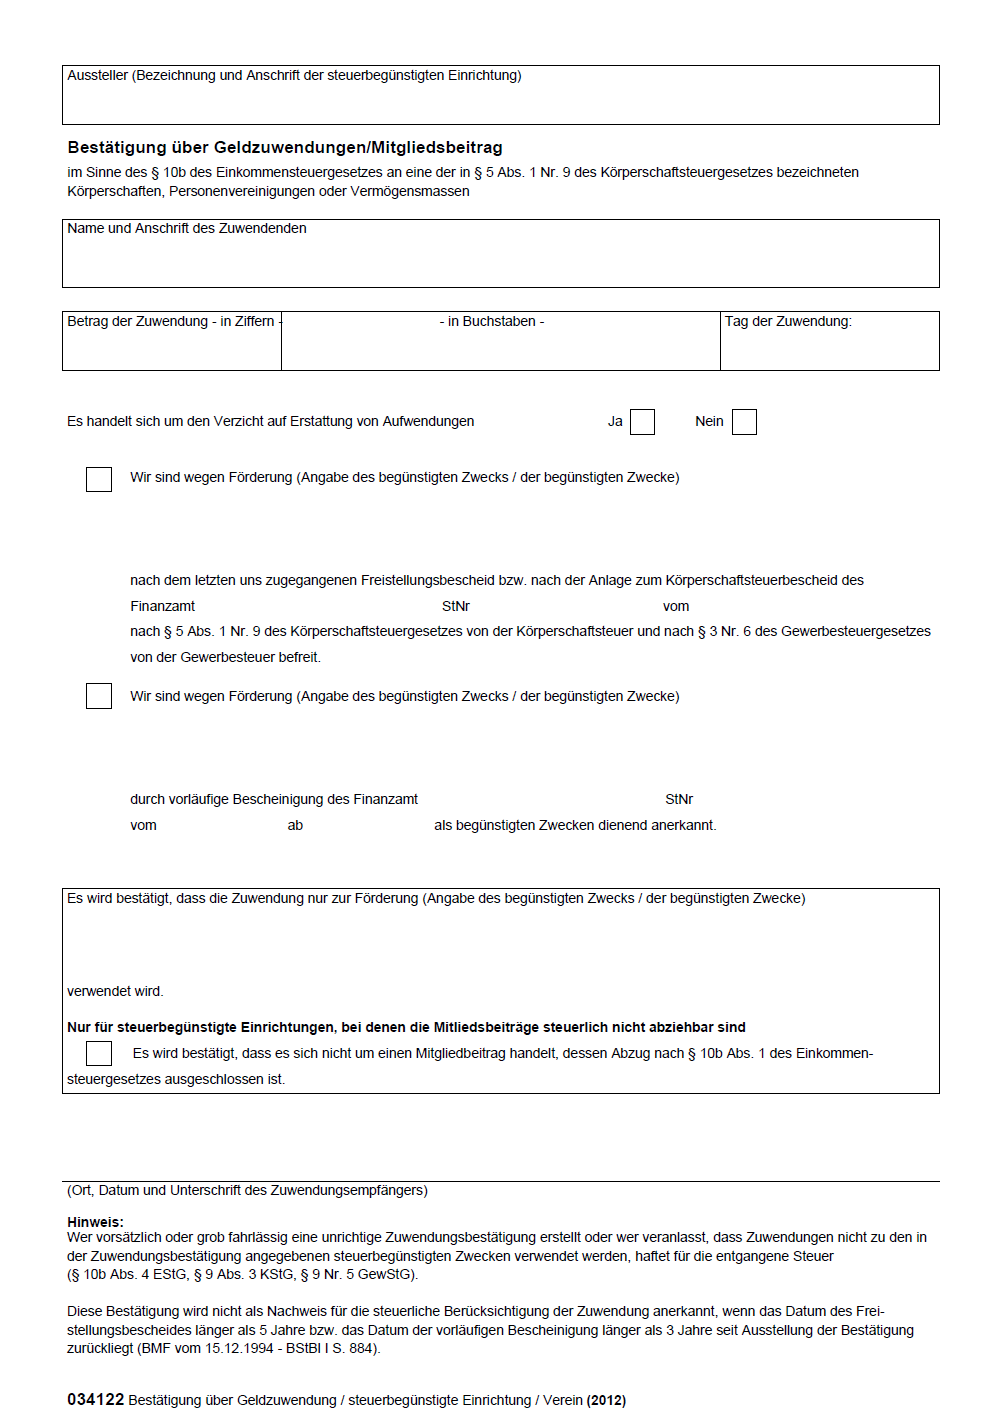
\includegraphics[width=0.75\textwidth]{01_Geldzuwendungen-Mitgliedsbeitrag-10b}}
\caption{Spendenformular, {\footnotesize Quelle: \texttt{http://www.finanzamt.bayern.de}}}\label{fig:original}
\end{center}
\end{figure}


\begin{figure}[h]
\begin{center}
\fbox{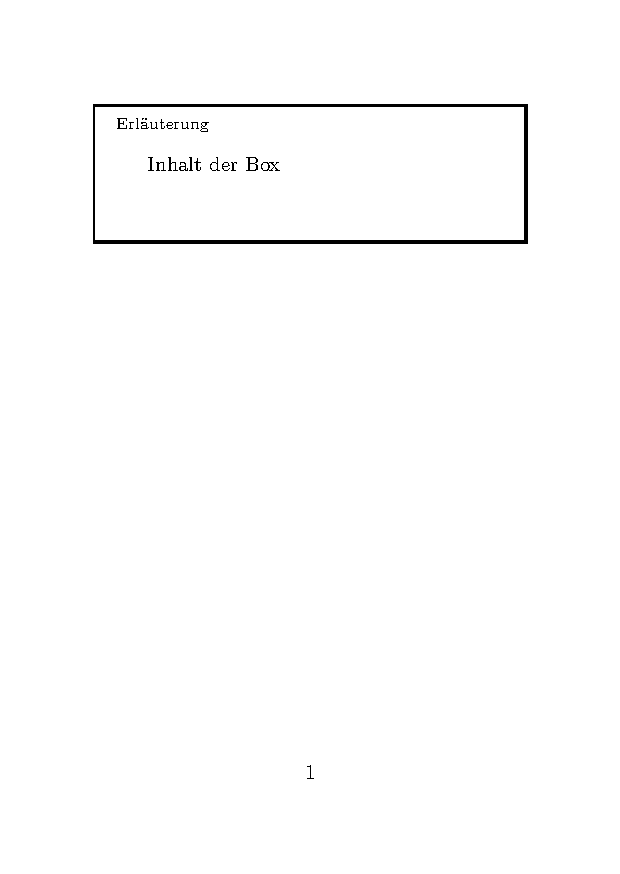
\includegraphics[width=0.75\textwidth]{mdf-heidelberg}}
\caption{Ergebnis von Listing \ref{lis:mdf}}\label{fig:mdf}
\end{center}
\end{figure}

Eine weitere Herausforderung war das Ausschreiben des gespendeten Betrags als Wort. Hier hätte Nicola Talbots \texttt{fmtcount} Paket \cite{fmtcount} sehr nützlich können, dessen \verb|\Numberstringnum| Befehl eine ganze Zahl (ohne Dezimalteil) entgegennimmt und die textliche Repräsentation als Zeichenkette zurückgibt. 
Leider kann das Paket mit den im Deutschen anzutreffenden Sprach-Feinheiten nicht umgehen, so wird aus \enquote{123} \enquote{Einshundertdreiundzwanzig} statt \enquote{Einhundertdreiundzwanzig}. 

Die finale Lösung bestand dann darin, eine weitere Tabelle in der Datenbank mit fertigen Zahlwörtern für jeden ganzzahligen Betrag zwischen 1 und 9999 zu befüllen und diese weiteren Programmablauf auszuwerten.

\section{Erstellung der Datenbankabfragen}

Nach der Erstellung des Layouts war es nun Zeit, die gewohnten \LaTeX-Pfade zu verlassen, um die Daten für die Spendenquittungen aufzubereiten. 

Zum Skripten der verschiedenen benötigten Funktionen wurde Python genutzt, das sich bei mir persönlich durch einen hohen Funktionsumfang bei  guter Lesbarkeit des Quellcodes und leichter Erlernbarkeit beliebt gemacht hat. 

Die Buchungen der Dingfabrik werden in Lexware Quicken verwaltet, das neben seiner wichtigsten Funktion -- dem Abholen der Kontoauszüge von der Bank mittels HBCI -- verschiedene Möglichkeiten zur Klassifikation und Auswertung der Daten bietet. 

Aus Quicken werden die klassifizierten Buchungen dann für die Weiterverarbeitung exportiert.
Der CSV-Export\footnote{Comma-Separated Values} aus Quicken heraus war leider unbrauchbar, da die Daten im CP1252 (Latin1) Encoding ausgegeben wurden und erste Versuche, die Daten mittels Python einzulesen, in defekten Umlauten resultierten.

Der Excel-Export war deutlich besser zu nutzen, da Excel schon seit mehreren Version alle Daten in Unicode abspeichert. Wirklich \enquote{perfekt} ist jedoch auch dieser Export nicht, da Quicken in den ersten und letzten Zeilen des entsprechenden Arbeitsblattes verschiedene Meta-Informationen einfügt, die sich auch nicht wegkonfigurieren lassen.

\begin{lstlisting}[frame=single,caption={Python Quellcode zum Auslesen von Excel-Daten},language={Python},label={lis:xlrd},morekeywords={xlrd,open_workbook,sheet_by_name,sheet_names,nrows,ncols}]
import xlrd
workbook = xlrd.open_workbook('Buchungen_20131129.xlsx')
worksheet = workbook.sheet_by_name('Sheet')
num_rows =  worksheet.nrows - 10
num_cells = worksheet.ncols - 1
curr_row = 8

while curr_row < num_rows:
	curr_row += 1
	datum = str(worksheet.cell_value(curr_row, 1))
	beschreibung = worksheet.cell_value(curr_row, 5)
	zweck = worksheet.cell_value(curr_row, 5)
	kategorie = worksheet.cell_value(curr_row, 6)
	klasse = worksheet.cell_value(curr_row, 7)
	betrag = worksheet.cell_value(curr_row, 9)
	print(datum, " ", beschreibung," ", zweck," ", kategorie," ", betrag)
\end{lstlisting}

Das von mir genutzte Python-Modul \texttt{xlrd} \cite{xlrd} verfügt jedoch  über entsprechende Funktionen, den auszulesenden Teil einer Excel-Datei genau zu definieren. Listing~\ref{lis:xlrd} zeigt ein Beispiel von der \texttt{xlrd}-Webseite, das etwas angepasst wurde, um die Daten aus der exportierten Quicken-Datei \enquote{Buchungen.xlsx} auszulesen.

Das Auslesen der Daten aus Excel ist jedoch nur der erste Schritt, im nächsten Schritt werden die ausgelesenen Daten in eine Datenbank geschrieben, um die Daten mit SQL-Abfragen passend aufzubereiten und zu extrahieren.

Anfänglich habe ich SQLite genutzt, da Python dieses nicht nur standardmäßig mitbringt, es leicht zu konfigurieren ist, und sogenannte \enquote{In-Memory} Datenbanken unterstützt. 
\enquote{In-Memory} bedeutet, dass keine Datenbank-Datei auf der Dateiablage angelegt werden muss, alle Daten landen im Arbeitsspeicher.  

Dies bedeutet zwar, dass sie nach dem Lauf des Python-Skripts verloren sind, da die Datenmenge in meinem Anwendungsfall überschaubar groß ist und keine Persistenz der Daten über den Python-Lauf hinweg benötigt wird, war \enquote{In-Memory} hier vollkommen ausreichend. 

Im Laufe des Projekts kam noch der Wunsch nach der Verbindung zu den Stammdaten auf, die in MySQL gehalten werden, aus Gründen der Vereinheitlichung wurde daher auf MySQL umgestellt. Als Datenbank-Treiber diente das offizielle von Oracle angebotene Python Modul\footnote{\url{http://dev.mysql.com/downloads/connector/python}}.



\begin{lstlisting}[frame=single,caption={Python Quellcode für eine MySQL Datenbank},language={Python},label={lis:sql1},morekeywords={cursor,connect,execute,fetchall,commit,close}]
import mysql.connector

db = mysql.connector.connect(host="localhost",user="root",
                      passwd="uweuwe", db="TestDB")

cur = db.cursor() 
cur.execute("insert into test values('Max','Hase')")
db.commit()
cur.execute("SELECT * FROM test")

for row in cur.fetchall():
    print (row)
\end{lstlisting}

Listing \ref{lis:sql1} zeigt ein einfaches Beispiel, wie man mit Python Daten in eine MySQL Datenbank schreiben und auch wieder auslesen kann. 

Mehr zum Thema SQLite und MySQL findet man beispielsweise unter \cite{sqlite} oder in \cite{pypro}.

Über eine Kombination der Skripte aus den Listings \ref{lis:xlrd} und \ref{lis:sql1} wurden dann die Kontoauszüge aus der Excel-Datei in die MySQL Datenbank geladen, weitere SQL Statements holen die Daten dann auch wieder aus der Datenbank, um sie in die \LaTeX\ Dokumente einzufügen.

\section{Erzeugen der Dokumente}

Für die Kombination des \LaTeX-Dokuments mit den SQL-Daten nutze ich \texttt{Jinja2}, eine auf Python basierende Template-Engine. 

Template Engines machen nichts anderes, als in einer Vorlage bestimmte Platzhalter mit Werten zu ersetzen. Dies lässt sich zwar auch mit Bordmitteln erreichen, Template Engines sind aber üblicherweise deutlich schneller  und der Quellcode bleibt eleganter und übersichtlicher.

Python besitzt zwar seit Version 2.4 auch eine eingebaute Template Engine, Jinja2 bietet jedoch noch einige nützliche Zusatzfunktionen wie eine eingebaute Skriptsprache, mit der z.\,B. Aufzählungen oder Tabellenzeilen recht einfach gesetzt werden können.
 

\begin{lstlisting}[frame=single,caption={\texttt{Jinja2} Beispiel},language={Python},label={lis:jinja2},morekeywords={Environment,block_start_string,%
block_end_string,variable_start_string,variable_end_string,comment_start_string,comment_end_string,%
line_statement_prefix,line_comment_prefix,trim_blocks,autoescape,loader,path,abspath,FileSystemLoader,%
get_template,render}]
import jinja2 
import os

latex_jinja_env = jinja2.Environment(
    block_start_string = '\BLOCK{',
    block_end_string = '}',
    variable_start_string = '\VAR{',
    variable_end_string = '}',
    comment_start_string = '\#{',
    comment_end_string = '}',
    line_statement_prefix = '%-',
    line_comment_prefix = '%#',
    trim_blocks = True,
    autoescape = False,
    loader = jinja2.FileSystemLoader(os.path.abspath('.'))
)
\end{lstlisting}

Jinja2 nutzt standardmäßig doppelte geschweifte Klammern zur Kennzeichnung von Platzhaltern, die bekanntermaßen auch in \LaTeX\ eine zentrale Rolle spielen. Listing \ref{lis:jinja2} zeigt daher ein entsprechendes Minimalbeispiel, das zuerst \LaTeX-Kompatibilität\footnote{Code urprünglich von \url{http://e6h.de/post/11/}} sowie die Funktionalität zum Laden von Vorlagen aus Dateien herstellt.


Aus der Beispieldatei von Listing \ref{lis:jj2item} wird beim Python-Lauf der \LaTeX-Code von Listing \ref{lis:jinja2out} erzeugt,
Damit haben wir nun alles an Funktionalität, was wir im weiteren Verlauf für unsere \LaTeX-Dokumente benötigt wird.

Die Vorlage für die Spendenquittung wird im nächsten Schritt um die Jinja2-Variablen erweitert und mit dem Datenbank-Code verbunden.


\begin{lstlisting}[frame=single,caption={Beispieldatei \texttt{test-itemize.tex} für Jinja2},language={[LaTeX]TeX},morekeywords={VAR,BLOCK},label={lis:jj2item}]
\section{\VAR{headline}}

\begin{itemize}
\BLOCK{for item in liste}
 \item \VAR{item}
\BLOCK{endfor}
\end{itemize}
\end{lstlisting}

\begin{lstlisting}[frame=single,caption={Ausgabe von Listing \ref{lis:jinja2}, generierter \LaTeX-Code} ,language={[LaTeX]TeX},morekeywords={VAR,BLOCK},label={lis:jinja2out}]
\section{Hello}

\begin{itemize}
 \item first
 \item second
 \item third
\end{itemize}
\end{lstlisting}

Auf den Abdruck des kompletten Quellcodes für das finale Skript (80 Zeilen) soll an dieser Stelle verzichtet werden, der geneigte Leser findet ihn zusammen mit den anderen Python-Skripten und Beschreibungen unter  \url{http://code.google.com/p/spendenquittungen-mit-latex/}. 

\clearpage
\section{Fazit}

Die vorgestellte Lösung vereint die elegante Mächtigkeit von Python mit \LaTeX, um mit -- im Vergleich zur manuellen Erstellung von mehreren Dutzend Spendenbescheinigungen -- recht geringem Aufwand professionelle Dokumente automatisiert erstellen zu können.

Für Feedback, Ideen und Wünsche bin ich dankbar.

\begin{thebibliography}{40}
\bibitem{esopic} Rolf Niepraschk, \enquote{eso-pic}, \url{http://www.ctan.org/pkg/eso-pic}
\bibitem{mdframed} Marco Daniel/Elke Schuber, \enquote{mdframed}, \url{http://www.ctan.org/pkg/mdframed}
\bibitem{xlrd} \url{http://www.python-excel.org}
\bibitem{sqlite} \url{http://www.zetcode.com/db/sqlitepythontutorial/}
\bibitem{pypro} Mark Lutz, \enquote{Programming Python}, O'Reilly
\bibitem{forms} Uwe Ziegenhagen, \enquote{Formulare ausfüllen mit \LaTeX}, \url{http://uweziegenhagen.de/?p=1402}
\bibitem{fmtcount} Nicola Talbot, \enquote{fmtcount}, \url{http://www.ctan.org/pkg/fmtcount}
\end{thebibliography}

\end{document}